\FloatBarrier
\section{Cherenkov Radiation and Detectors}\label{sec:clas.cc}

When a charged particle traverses through a medium with a velocity less than the speed of light for that medium ($v < c/n$) the dipoles of the molecules in the medium are symmetrically arranged such that the integrated dipole field along the particles path vanishes. However, when the particles speed is greater than that of the speed of light for that medium the dipoles of the molecules arrange themselves such that they are asymmetric along the particles path and thus creates a dipole field, see Fig~\ref{fig:clas.cc.dipole}.
\begin{figure}[h!]\begin{center}
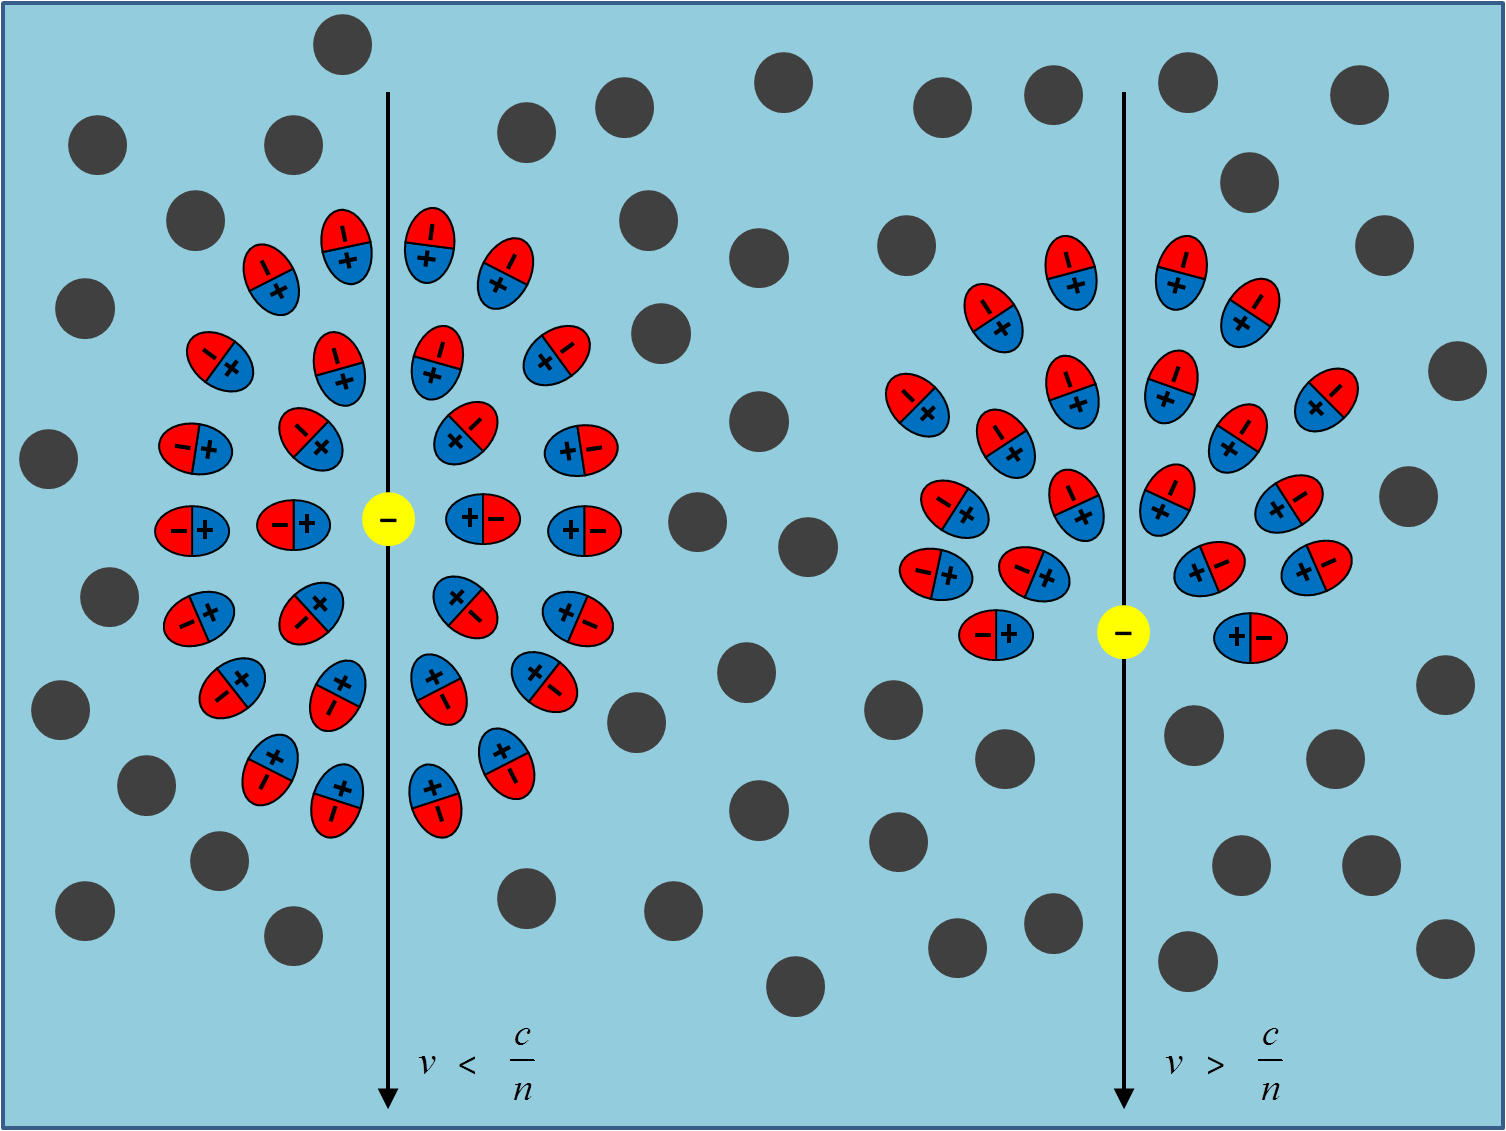
\includegraphics[width=\figwidth,height=\qfigheight]{\figures/hall-b/CCECPLOTS/cherenkov.pdf}
\caption[Illustration of Cherenkov Radiation]{\label{fig:clas.cc.dipole}Illustration of Cherenkov Radiation. Negative charged particle traveling through a medium with $v < c/n$ showing dipoles symmetrically arranged around particles path (left). Negative charged particle traveling through a medium with $v > c/n$ showing dipoles asymmetrically arranged around particles path given rise to dipole field(right). Image Source:~\cite{cherenkov_image}}
\end{center}\end{figure}

The generated dipole field radiates the energy contained in this disturbance producing a coherent shockwave, this is known as Cherenkov radiation. An analogy of this phenomena is the sonic boom created in air from an object traveling faster then the speed of sound. Just as the sound wave of a sonic boom travels slower than the traveling object, so does the light emitted from the dipole field. This reduction in velocity creates the wave front of a continuous light spectrum, see Fig~\ref{fig:clas.cc.angle}.
\begin{figure}[h!]\begin{center}
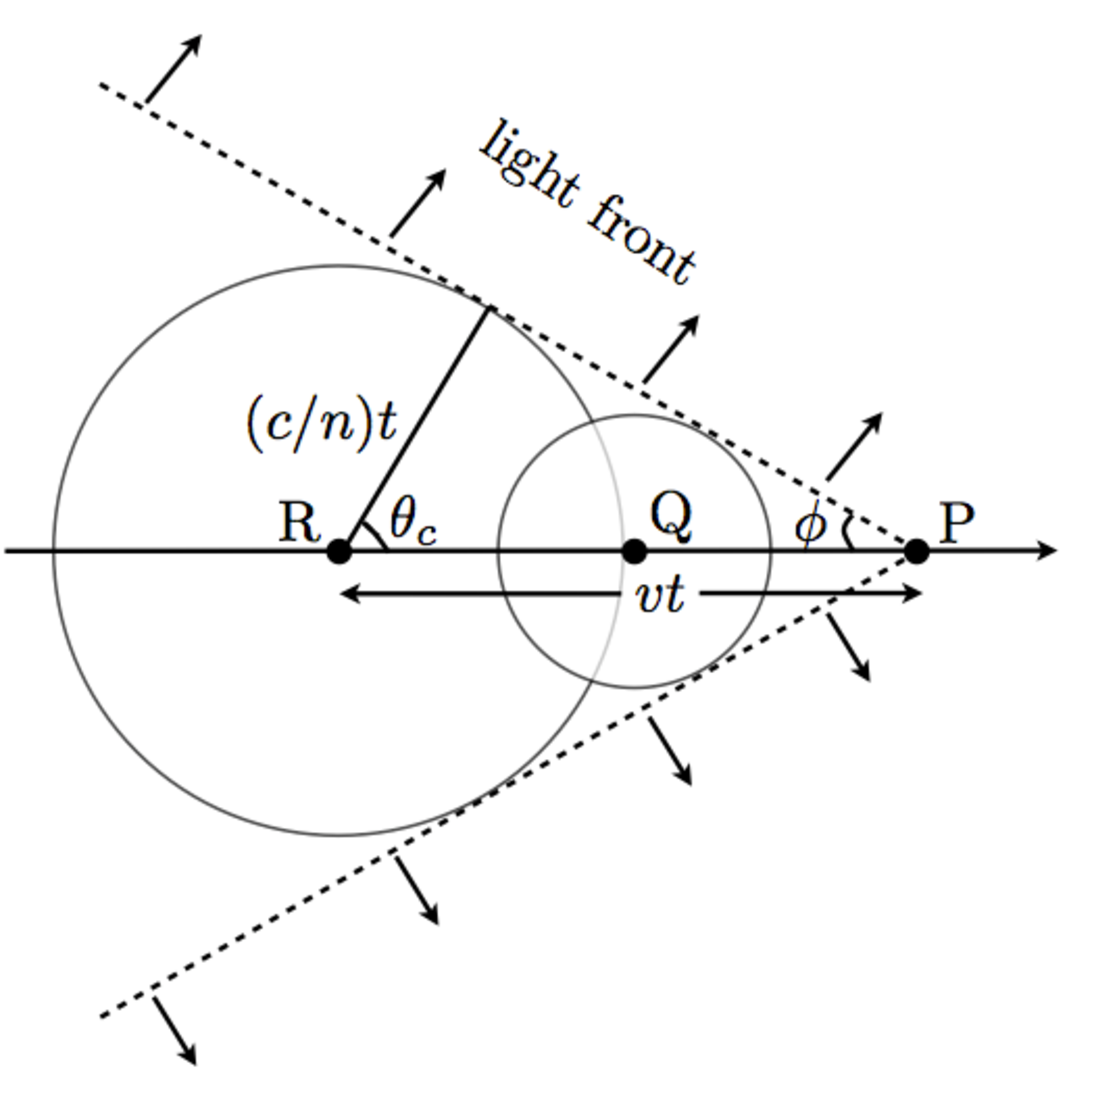
\includegraphics[width=\figwidth,height=0.75\hfigheight]{\figures/hall-b/CCECPLOTS/cc_wavefront_madeII.pdf}
\caption[Illustration of Cherenkov Angle]{\label{fig:clas.cc.angle}Illustration of Cherenkov Angle. When the particle has traveled the distance $\mathrm{RP =\nu t \rightarrow \beta c t}$, the photon (light front) has traveled $(c/n)t$.}
\end{center}\end{figure}

Inspecting Fig~\ref{fig:clas.cc.angle}, when the particle has traveled the distance $\mathrm{RP =\nu t = t \beta c}$, the photon has traveled $(c/n)t$, therefore
\begin{equation}\label{eq:cherenkov_eq}
 \mathrm{\cos\theta_{c} = \frac{(c/n)t}{t \beta c} = \frac{1}{n\beta}}
\end{equation}
and the threshold of Cherenkov radiation is 
\begin{equation}\label{eq:cherenkov_threshold}
 \mathrm{\beta_{th} > \frac{1}{n}}.
\end{equation}
Adding in quantum effects
\begin{equation}\label{eq:cherenkov_eq_quantum}
\mathrm{cos\theta_{c} = \frac{1}{n\beta} + \frac{\Lambda}{\lambda}\frac{n^{2} -1}{2n^{2}}}
\end{equation}
where
\begin{equation}\label{eq:cherenkov_eq_quantum_lambda}
\mathrm{\Lambda = \frac{\sqrt{1-\beta^{2}}}{\beta}\lambda_{0}} \ , 
\end{equation}
$\mathrm{\lambda =}$ wavelength of light in medium, and $\mathrm{\lambda_{0} }$ is the Compton wavelength 0.024 \AA. For practical cases, and using \abbr{CLAS}, the 2$^{nd}$ order term is negligible (n=1.00153). To illustrate that quantum effects are negligible, an electron traveling at threshold in \abbr{CLAS} \abbr{CC},
\begin{equation}
\mathrm{\beta_{th} > \frac{1}{n}} > 0.998472,
\end{equation}

\begin{equation}
\mathrm{\frac{\Lambda}{\lambda}\frac{n^{2} -1}{2n^{2}} =  1.07874 \cdot 10^{-9}}
\end{equation}
%

In \abbr{CLAS}, the Cherenkov counter (\abbr{CC}) is used to detect electrons and positrons while rejecting pions for momenta less than 2.5~GeV. The gas used in the \abbr{CC} for \g12 is perfluorobutane (C$_4$F$_{10}$) with an index of refraction of 1.00153. The threshold energy for producing Cherenkov radiation in C$_4$F$_{10}$ is
\begin{align}
\mathrm{E_{th} = \gamma_{th} m_{0}} \mathrm{ \ (Units \ of \ c)} \\
\mathrm{\gamma_{th} = \frac{n}{\sqrt{n^{2} -1}}} = 18.09
\end{align}
therefore the threshold energy of e$^{\pm}$ is 9.23~MeV while the threshold energy of $\pi^{\pm}$ is 2.52~GeV.
%
The number of photons emitted per unit length at threshold for electrons or positrons is;
\begin{align}\label{eq:cc.NPE}
\frac{dN}{dx} = 2\pi z^2 \alpha \frac{\sin \theta_{c}^2}{\lambda^2} d\lambda = 0.241246 \frac{d\lambda}{\lambda^2}
\end{align}
where $\alpha$ is the fine structure constant, $z =1$ for electrons and positrons, and $\lambda$ is the wavelength at which the photon is emitted. Table~\ref{tab:cc_npe} lists the number of photons/cm for various wavelengths of light for the midpoint of $\beta_{th}$ and a maximum velocity $\beta =1$. Table~\ref{tab:cc_npe} also lists the mirror reflectivity for that wavelength.
\begin{table}[h!]
\begin{minipage}{\textwidth}
\begin{center}
\begin{singlespacing}

\caption[Number of Photo-electrons per Unit Length in Cherenkov Detection]{\label{tab:cc_npe}Number of $\gamma$'s per unit length gas $C_4F_10$ \vspace{0.75mm}}

\begin{tabular}{c|c|c|c}

\hline
Wavelength~nm & \multicolumn{2}{c|}{$\frac{dN}{dx}$~photons/cm} & Mirror reflectivity~\cite{clas.cc}  \vspace{0.5mm} \\
\hline
&$\beta = \frac{1}{2}(1+\beta_{th})$& $\beta = 1$ \\
\hline
400-700 (visible) & $0.75$ & $1.5$ & 90\% \\
300-400 (near UV) & $0.6$ & $1.2$ & 85 - 90 \% \\
190-300 (near UV) & $1.4$ & $2.7$ & 20 - 85\% \\
\hline \hline
\end{tabular}
\end{singlespacing}
\end{center}
\end{minipage}
\end{table}
\vspace{20pt}


The \abbr{CC} subsystem is physically located in the space between Region 3 of the \abbr{DC} subsystem and the \abbr{TOF} in the forward region covering polar angles 8$^\circ$ to 45$^\circ$ in each sector when the target is at \abbr{CLAS} center. For \g12 since the target was placed 90~cm upstream, the polar coverage was approximately from 6$^\circ$ to 35$^\circ$ in the lab frame. The \abbr{CLAS} \abbr{CC}'s were fabricated as 6 independent identical sectors, with each sector divided into 18 regions of $\mathrm{\theta}$, and each $\mathrm{\theta}$ segment divided into 2 modules. Light from Cherenkov radiation is focused in $\mathrm{\phi}$ thus preserving information on the lepton polar angle $\theta$. The optical element of \abbr{CC} module comprises an assembly of one elliptical and one hyperbolic mirror providing primary light focusing into a  ``Winston" light collection cone, a  cylindrical mirror used to compensate for imperfections in the focusing, and a photomultiplier used to count the  number of photons in the light cone, see Fig~\ref{fig:clas.cc_array}. More information on the \abbr{CLAS} Cherenkov detector can be found in~\cite{clas.cc} 

The use of the \abbr{CC} was not included in the original proposals, however a significant drop in price on C$_4$F$_{10}$ just prior to the start of \g12 allowed the gas to be added at the last minute. The price drop was due to the recent availability of another, much cheaper gas that was demonstrated to have the same general properties as C$_4$F$_{10}$ and when \g12 contacted the original supplier of the C$_4$F$_{10}$ for a price match, they committed. 

\begin{figure}[h!]\begin{center}
\subfloat[]{
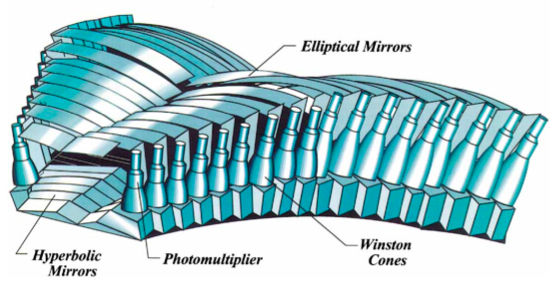
\includegraphics[width=\figwidth,height=0.5\hfigheight]{\figures/hall-b/CCECPLOTS/CCarray}\label{fig:clas.cc_array}
}\\
%[Schematic of one \abbr{CC} showing the 18 symmetrical, mirrored segments of the CLAS \abbr{CC}]
\subfloat[]{
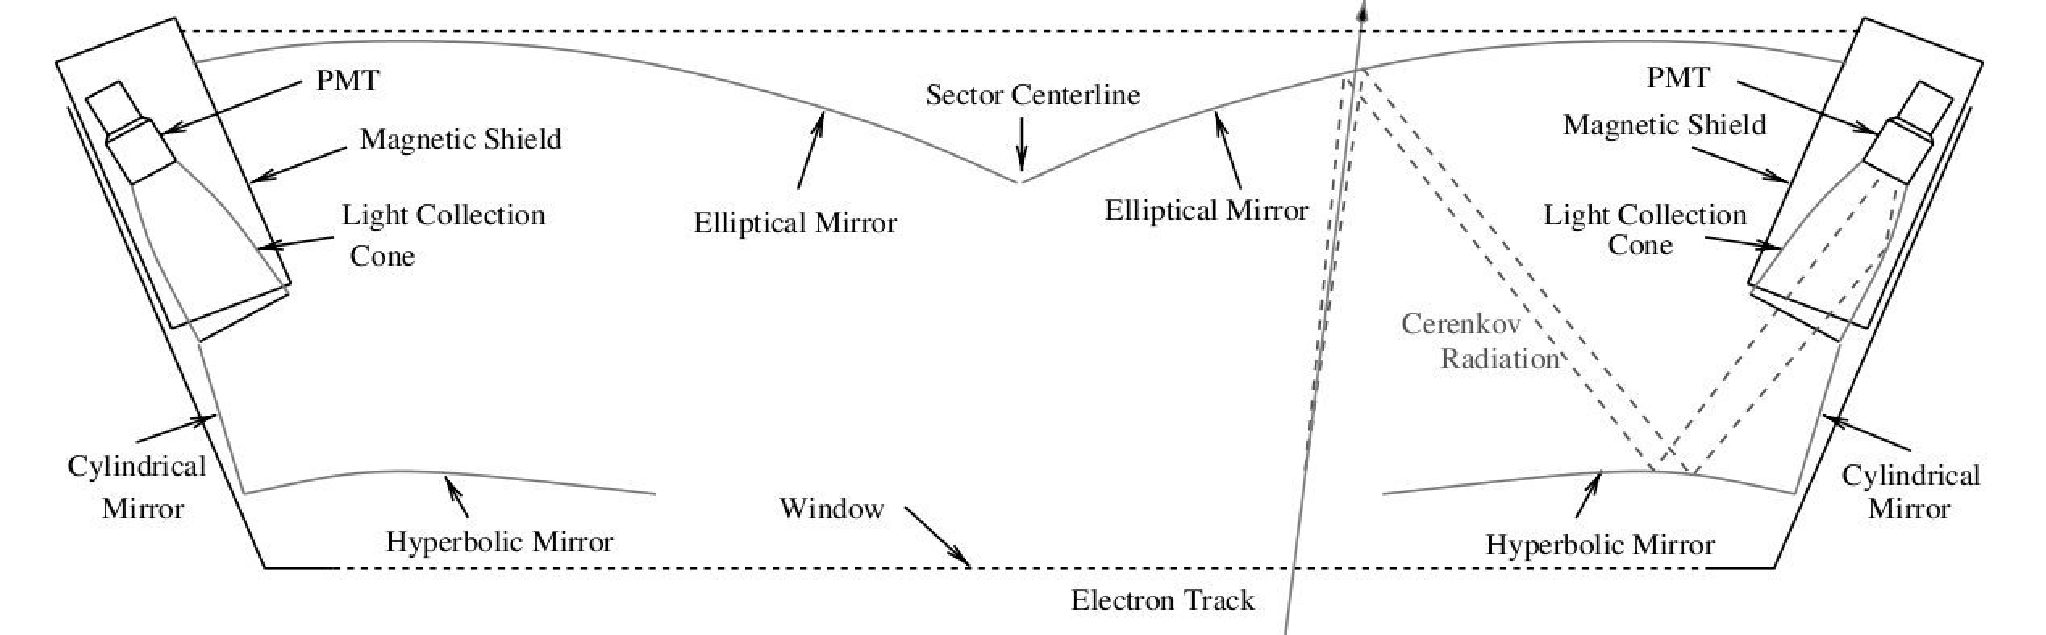
\includegraphics[width=0.9\columnwidth]{\figures/hall-b/cc_diagram.pdf}\label{fig:clas.cc}
}
\caption[Schematic of one \abbr{CC} showing the 18 symmetrical, mirrored segments of the CLAS \abbr{CC}]{Schematic of one \abbr{CC} showing the 18 symmetrical, mirrored segments of the CLAS \abbr{CC}~(a). Diagram of one segment of the Cherenkov counters with an electron entering from the bottom~(b).}

\end{center}\end{figure}





